% Created 2021-09-24 sex 17:31
% Intended LaTeX compiler: pdflatex
\documentclass[11pt]{article}
\usepackage[utf8]{inputenc}
\usepackage[T1]{fontenc}
\usepackage{graphicx}
\usepackage{grffile}
\usepackage{longtable}
\usepackage{wrapfig}
\usepackage{rotating}
\usepackage[normalem]{ulem}
\usepackage{amsmath}
\usepackage{textcomp}
\usepackage{amssymb}
\usepackage{capt-of}
\usepackage{hyperref}
\author{Filipe Gonçalves Jacinto}
\date{24 de Setembro de 2021}
\title{Análise de caso: Decomposição elétrica do TiS3 em condições ambientais através do método de Monte Carlo Cinético}
\hypersetup{
 pdfauthor={Filipe Gonçalves Jacinto},
 pdftitle={Análise de caso: Decomposição elétrica do TiS3 em condições ambientais através do método de Monte Carlo Cinético},
 pdfkeywords={},
 pdfsubject={Projeto que mostra que a perda de Enxofre(S) desempenha um papel importante na decomposição elétrica do TiS3 em condições ambientais},
 pdfcreator={Emacs 27.2 (Org mode 9.5)}, 
 pdflang={English}}
\begin{document}

\maketitle
\tableofcontents




\section{Introdução:}
\label{sec:org66f42fb}
Desde a síntese do Grafeno \cite{geim2010rise} materiais bidimensionais(2D) vem se mos- \linebreak trando como promissores candidatos para substituir os semicondutores convencionais baseados em Silício à medida em que se reduz a escala de dispositivos eletrônicos. Nesse sentido, são necessárias investigações mais profundas de materiais como o do \(TiS_3\) (Trissulfeto de Titânio) que possuem algumas características como um  \textit{Gap} de \(1~eV\) e pode ser isolado em monocamadas e nanotubos \cite{molina2017high}.

O artigo indicado pelo professor da disciplina de Física computacional \cite{molina2017high} discute as propriedades de decomposição elétrica do \(TiS_3\). Os resultados que foram obtidos de forma experimental e através de simulações computacionais sugerem que este fenômeno ocorre tanto devido a efeito Joule quanto por dessorção de moléculas de \(SO\) da superfície de \(TiS_3\) em uma atmosfera rica em \(O_2\) o que provoca a degradação do material e a consequente decomposição elétrica do \(TiS_3\) .

No contexto da disciplina de Física Computacional, este trabalho visa entender a dinâmica de dessorção de partículas no problema físico da decomposição elétrica do \(TiS_3\) em condições ambientais utilizando a linguagem Python e o Método de Monte Carlo Cinético (KMC) discutindo os resultados obtidos e comparando-os com o do artigo em questão\cite{molina2017high}. Além disso, deve ser também um manual básico de como o código desenvolvido funciona. Para isso, pretende-se utilizar alguns resultados ja disponibilizados pelo professor como as energias de formação de vacâncias calculadas utilizando o pacote Quantum Espresso\cite{giannozzi2009quantum} , e a termogravimetria disponibilizada no artigo\cite{molina2017high} para calcular a dinâmica de dessorção do \(S\) da monocamada de \(TiS_3\) rica em O\textsubscript{2} e compara-la com o experimento.


\section{Metodologia:}
\label{sec:org1f4cfe7}
\subsection{Algoritmo(KMC):}
\label{sec:orgaa56274}
Para estudar a dinâmica de dessorção do \(S\) da monocamada de \(TiS_3\) foram contruídos códigos em python utilizando a estrutura de algoritmo KMC em específico o método Bortz-Kalos-Lebowitz (BKL) que é utilizado para estudar a evolução no tempo de um sistema onde os processos podem ser estudados através de uma taxa conhecida nesse caso \(R_i\) e podem ser descritas ao longo do tempo através dos seguintes passos:
\begin{enumerate}
\item Fixar o o tempo inicial t = 0;
\item Criar uma lista com todas a probabilidades $\Delta_i$ do sistema;

    Este passo é extremamente importante, pois aqui esta uma parte da Física do sistema , os eventos $\Delta_i$ são as energias associadas a cada evento de dessorção descrito nas Tabelas~\ref{t1} e~\ref{t2}. Através de cada $\Delta_i$ pode-se calcular as probabilidades de ocorrência de cada evento ($\Gamma_i$) através da equação~\ref{eq1} onde $\Gamma_{i}^{0}= 10^{13}~s^{-1}$ e é a frequência de ocorrência de cada evento.
\begin{table}[ht]
\centering
\begin{tabular}{| l| l| l| l|}
\hline
\textbf{Evento} & \textbf{Sistema} & \textbf{Defeito} & \textbf{Energia (\textit{eV})}\\
\hline
\hline
1 & $TiS_3O_{0.50}$ & Defeito de $SO$ (primeiro)   & 1.23 \\
\hline
2 & $TiS_3O_{0.50}$ & Defeito de $SO$ + monovacância & 1.55 \\
\hline
3 & $TiS_3O_{0.50}$ & Defeito de $SO$ + monovacância& 1.63 \\
\hline
4 & $TiS_3O_{0.50}$ &  Defeito de $SO$ (divacância)& 2.61 \\
\hline
\end{tabular}
\caption{Tabela com a respectiva energia de ativação de cada evento para uma superfície com $50\%$ de Oxigênio.}
\label{t1}
\end{table}

\begin{table}[ht]
\centering
\begin{tabular}{| l| l| l| l|}
\hline
\textbf{Evento} & \textbf{Sistema} & \textbf{Defeito} & \textbf{Energia (\textit{eV})}\\
\hline
\hline
1 & $TiS_3O_{0.25}$ & Defeito de $SO$ (primeiro)   & 1.23 \\
\hline
2 & $TiS_3O_{0.25}$ & Defeito de $SO$ + monovacância & 1.51 \\
\hline
3 & $TiS_3O_{0.25}$ & Defeito de $SO$ + monovacância& 1.78 \\
\hline
4 & $TiS_3O_{0.25}$ &  Defeito de $SO$ (divacância)& 2.62 \\
\hline
\end{tabular}
\caption{Tabela com a respectiva energia de ativação de cada evento para uma superfície com $25\%$ de Oxigênio.}
\label{t2}
\end{table}



    \begin{equation}
        \Gamma_i = \Gamma_{i}^{0}\exp{\left({\frac{-\Delta_i}{K_b T}}\right)}
        \label{eq1}
    \end{equation}

\item Calcular a função acumulativa $R_n$ que é a soma da probabilidade acumulativa dos eventos que pode ser feita de acordo com a Equação~\ref{eq2} onde $R_i$ é a probabilidade de cada evento , $N_i$ número de partículas que podem realizar o i-ésimo evento e $n_e$ o número total de eventos considerados possíveis;

    \begin{equation}
        R_n = \sum_{i=1}^{n_e} R_i = \sum_{i=1}^{n_e} \Gamma_i N_i
        \label{eq2}
    \end{equation}

\item Gerar um número aleatório em relação a uma distribuição uniforme entre $u \in~(0,1]$;
\item Encontrar qual será a transição que ocorerá , ou seja, verificar qual termo da lista de probabilidade $R_i$ que respeita a condição da inequação~\ref{eq3}:
    \begin{equation}
    R_{i-1} < uR_n < R_i
    \label{eq3}
    \end{equation}

\item Realizar a transição. Este passo depende muito do sistema em questão, nesse caso em específico fazer a transição significa levar em conta a mudança na lista de partículas dos eventos possíveis e no caso da variação de temperatura calcular novamente os valores de $\Gamma$. Além disso, para calcular a massa perdida leva-se em conta que um evento para uma monovacância isto é o número de átomos diminui em um único átomo, já para o um divacância o número total de partículas será reduzido em dois.

\item Gerar um novo número aleatório em relação a uma distribuição uniforme entre $u \in~(0,1]$;
\item Realizar uma translação temporal $t \rightarrow t+\Delta t$ onde $\Delta t$ é dada pela equação~\ref{eq4}:
    \begin{equation}
        \Delta t = R^{-1} \ln{(1/u)}
        \label{eq4}
    \end{equation}

\item Atualizar a os valores de $R_i$ a partir das transição realizada e recalcular o valor de $R_n$;
\item Voltar ao passo 2.

\end{enumerate}


\subsection{Estrutura do código:}
\label{sec:orgd732bdd}
O código é estruturado em dois arquivos o \texttt{funcoes.py} e \texttt{main.py}. O arquivo de \texttt{funcoes.py} é onde estão escritas os passos do método de Monte Carlo na forma de funções e o arquivo \texttt{main.py} é o algoritmo estruturado na ordem correta com as funcões previamente escritas no arquivo \texttt{funcoes.py} .
\subsubsection{Pré-requisitos:}
\label{sec:org9b4e37d}
Para este código foi utilizado a linguagem Python 3.9.7, e os seguintes pacotes devem ser instalados com um gerenciador de pacotes de sua escolha, neste caso foi utilizado o \texbf{pip}. Para instalar os pacotes basta utilizar os comandos abaixo:

\begin{itemize}
\item \texttt{pip install matplotlib}
\item \texttt{pip install numpy}
\item \texttt{pip install scipy}
\item \texttt{pip install random}
\end{itemize}

\subsubsection{Arquivo 1:}
\label{sec:orgd035455}
As funções necessárias para implentar o método de KMC estão escritas no \texttt{funcoes.py} para que possam ser chamadas no arquivo principal \texttt{main.py}. Por isso, se faz necessário que este arquivo esteja sempre no mesmo diretório que o da função principal.
\begin{enumerate}
\item \texttt{Gamma}:
\label{sec:orgecd5235}
\begin{itemize}
\item Faz o cálculo de \texttt{Gamma[i]} ;
\item Soma \texttt{Gamma[i]} para obter o total \texttt{Gamma}.
\end{itemize}
\item \texttt{R\_sum}:
\label{sec:org3fc373b}
\begin{itemize}
\item Cálcula \texttt{R\_i}[i];
\item Soma os termos de \texttt{R\_i}[i] para obter \texttt{R\_n}.
\end{itemize}
\item \texttt{Probable\_event}:
\label{sec:orgc379912}
\begin{itemize}
\item Define qual foi o evento escolhido;
\item Realiza a transição.
\end{itemize}
\item \texttt{Time\_foward}:
\label{sec:orga695e11}
\begin{itemize}
\item Cálcula o \texttt{time\_step} (intervalo do evento) e o adiciona ao contador de tempo(t).
\end{itemize}
\item \texttt{Temp\_foward}:
\label{sec:org8842058}
\begin{itemize}
\item Cálcula o tempo transcorrido entre duas iterações consecutivas do método de KMC;
\item Em seguida cálcula o \texttt{temp\_step} proporcional a diferença de tempo transcorrida entre os passos dois passos consecutivos do método de KMC;
\item Adiciona o \texttt{temp\_step} ao contador de temperatura(T).
\end{itemize}
\end{enumerate}

\subsubsection{Arquivo 2: \texttt{main.py}}
\label{sec:orgc805b5f}
Este código é dividido em três partes sendo estas:
\begin{enumerate}
\item A primeira parte declara as variáveis e arrays necessários para esse algoritmo, em específico:

\begin{itemize}
\item \textbf{Variáveis}
\begin{itemize}
\item \texttt{gamma\_zero};
\item \texttt{temperatura};
\item \texttt{t} (tempo).
\end{itemize}
\item \textbf{Arrays}
\begin{itemize}
\item \texttt{Delta} (energias de ativação)
\item N(número de particulas que podem realizar o evento )
\end{itemize}
\item \textbf{Empty Arrays}
\begin{itemize}
\item \texttt{time} (armazena os tempos calculados em cada iteração)
\item \texttt{rate} (armazena a soma \texttt{R\_n} ao longo do tempo)
\end{itemize}
\end{itemize}
\item Esta parte é onde está estruturado a ordem do algoritmo utilizando as funções definidas em \texttt{funcoes.py}. O algoritmo segue a seguinte forma:
\begin{enumerate}
\item For in range(numero de iterações necessárias)
\begin{itemize}
\item Lista de eventos dentro do for:
\begin{enumerate}
\item \texttt{Gamma()} ;
\item \texttt{R\_sum()} ;
\item \texttt{Probable\_event()};
\item \texttt{Time Foward};
\item \texttt{Temp Foward}, no caso em que se varia a temperatura;
\item Adicionamos o termo no array de \textbf{time}
\item Adicionamos o termo no array de \textbf{mass}
\end{enumerate}
\end{itemize}
\end{enumerate}
\item A parte final do algoritmo consiste em plotar/calcular quantidades que ajudem a compreender o problema.Como por exemplo o plot de gráfico utilizando o pacote matplotlib.
\end{enumerate}



\section{Resultados e Discussão:}
\label{sec:org133e89a}
\begin{figure}[!htbp]
%\centering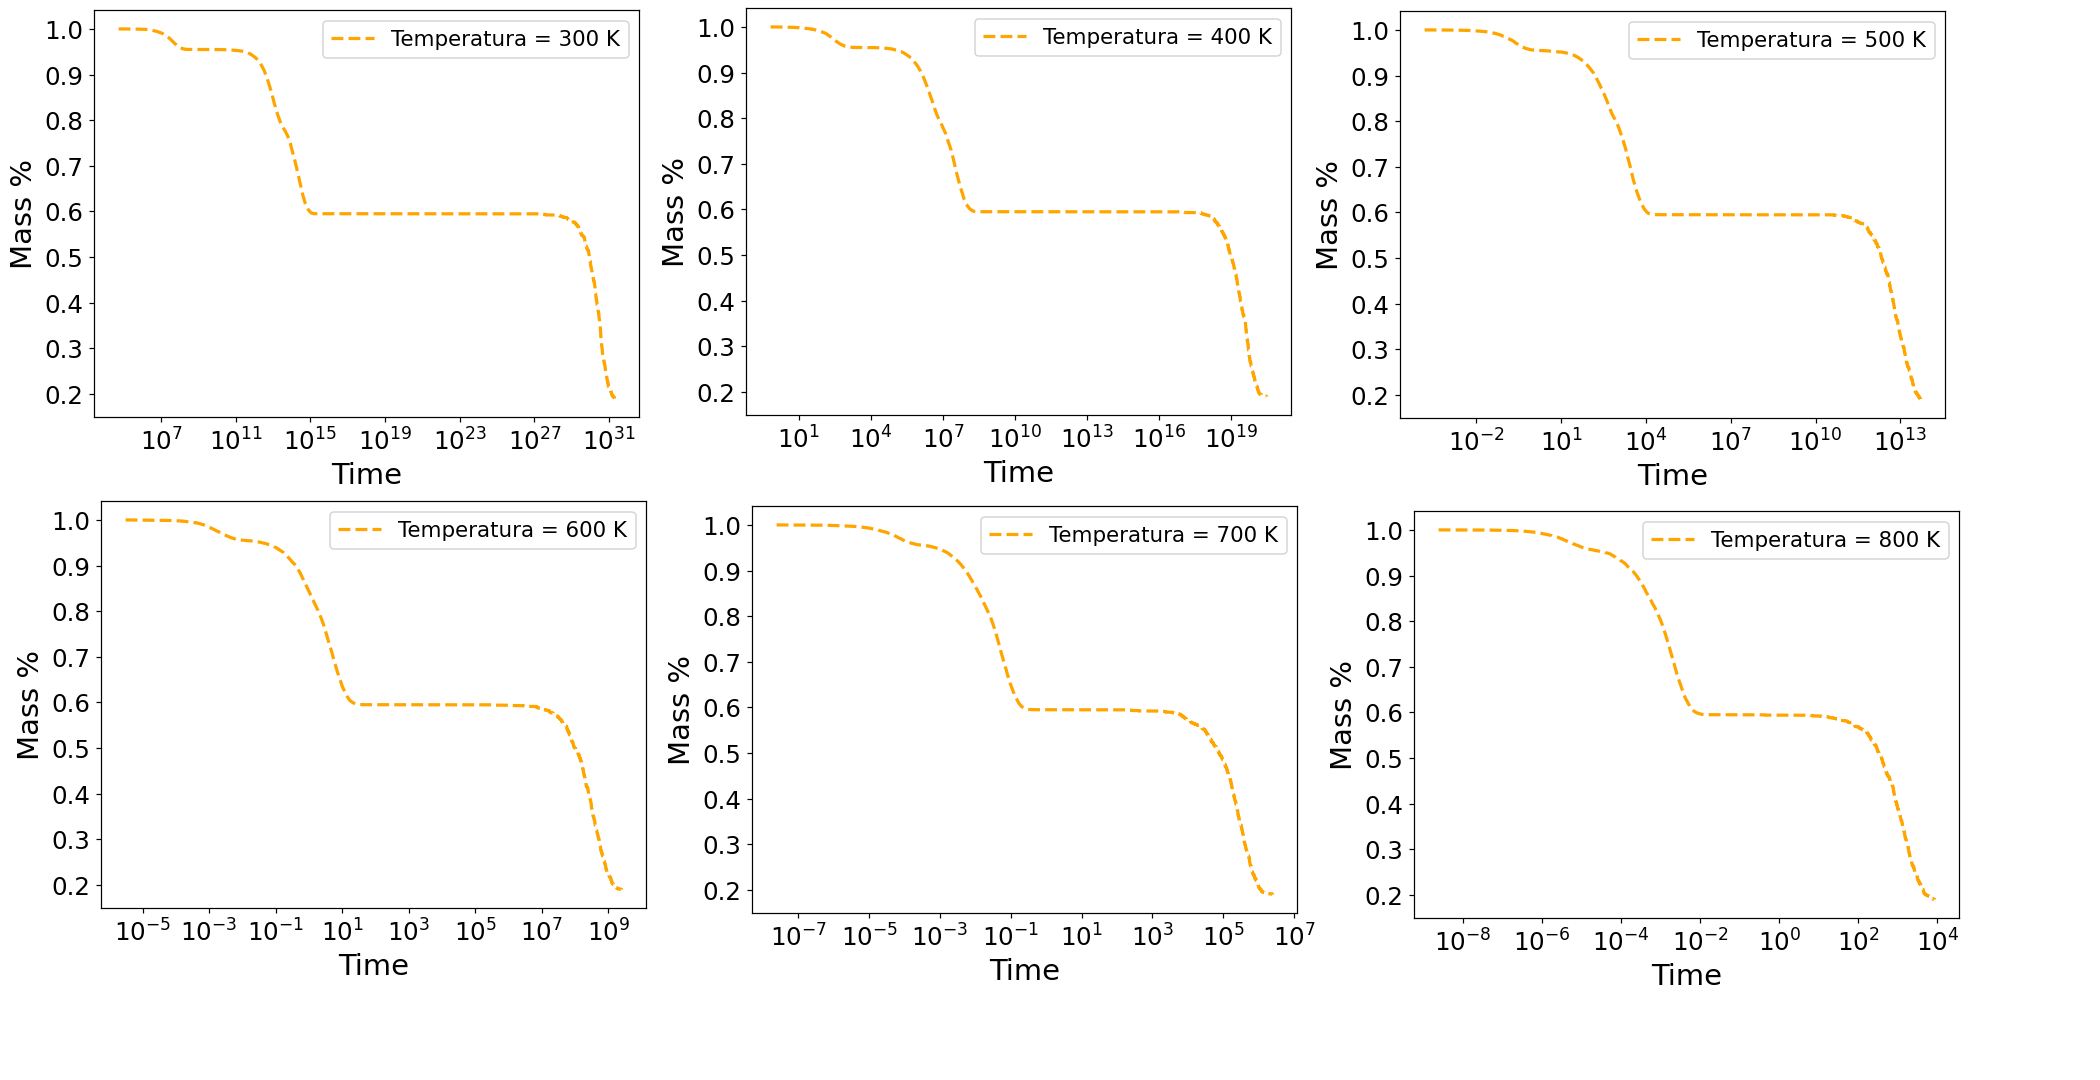
\includegraphics[width=1\linewidth]{figures/var-massa-tempo.png}
\centering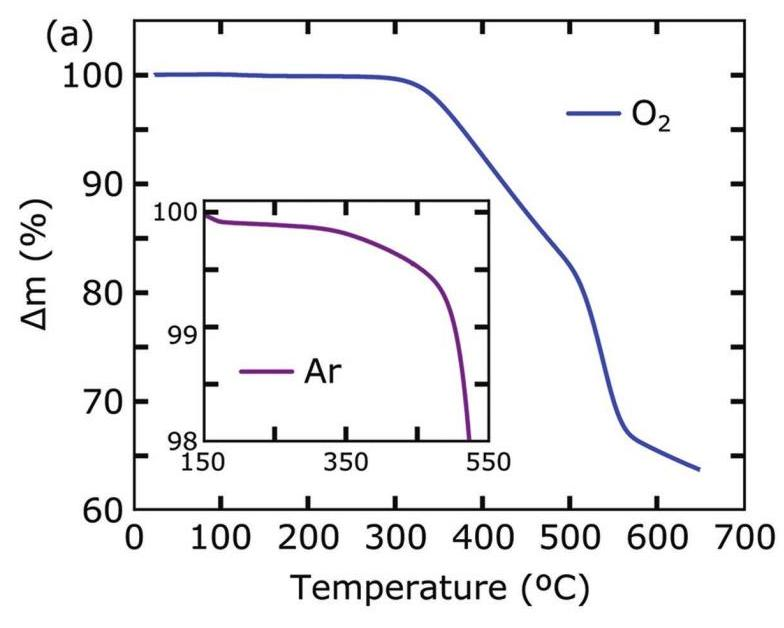
\includegraphics[scale=0.35]{figures/var-massa-temp.jpg}
\caption{Curva de termogravimetria para o \texit{bulk} de $TiS_3$ .}
\label{f1}
\end{figure}

De forma a estudar o papel da perda de massa do \(TiS_3\) no fenômeno de decomposição elétrica foram analisados resultados de alguns experimentos sendo um desses o de termogravimetria. A Figura \ref{f1} apresenta a curva de termogravimetria sob efeito de uma atmosfera rica em \(O_2\) obtida experimental- \linebreak mente\cite{molina2017high}. Observando a Figura \ref{f1}, pode-se ver uma variação de massa de \(36\%\) em um intervalo de temperatura de \(27~^\circ C\) até \(650~^\circ C\). Nesse intervalo de temperatura, pode-se notar dois eventos a citar: (1) no intervalo de  \(300-400~^\circ C\) com uma variação de massa de \(18\%\) e (2) no intervalo de \(450-550~^\circ C\) com uma variação de massa também de \(18\%\).


\begin{figure}[!htbp]
%\centering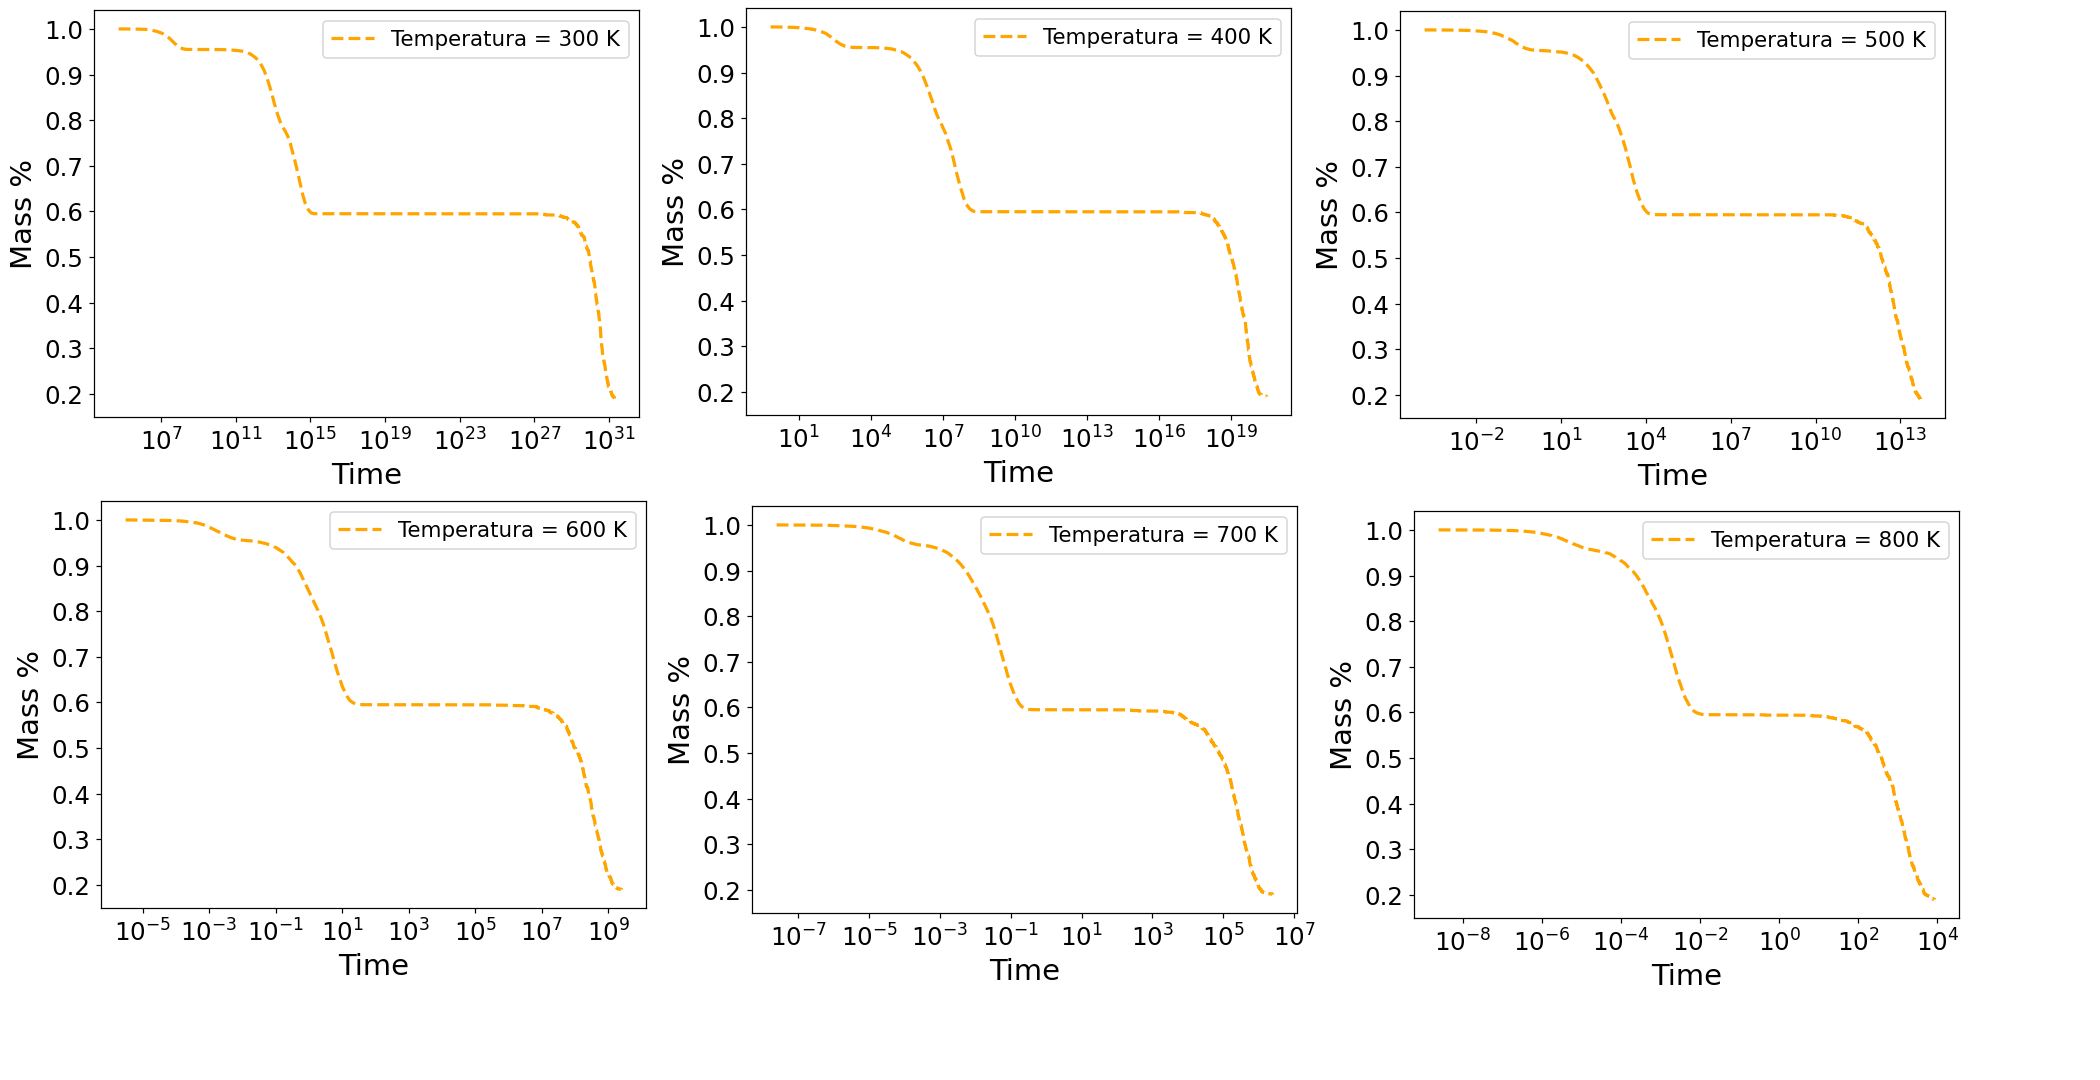
\includegraphics[width=1\linewidth]{figures/var-massa-tempo.png}
\centering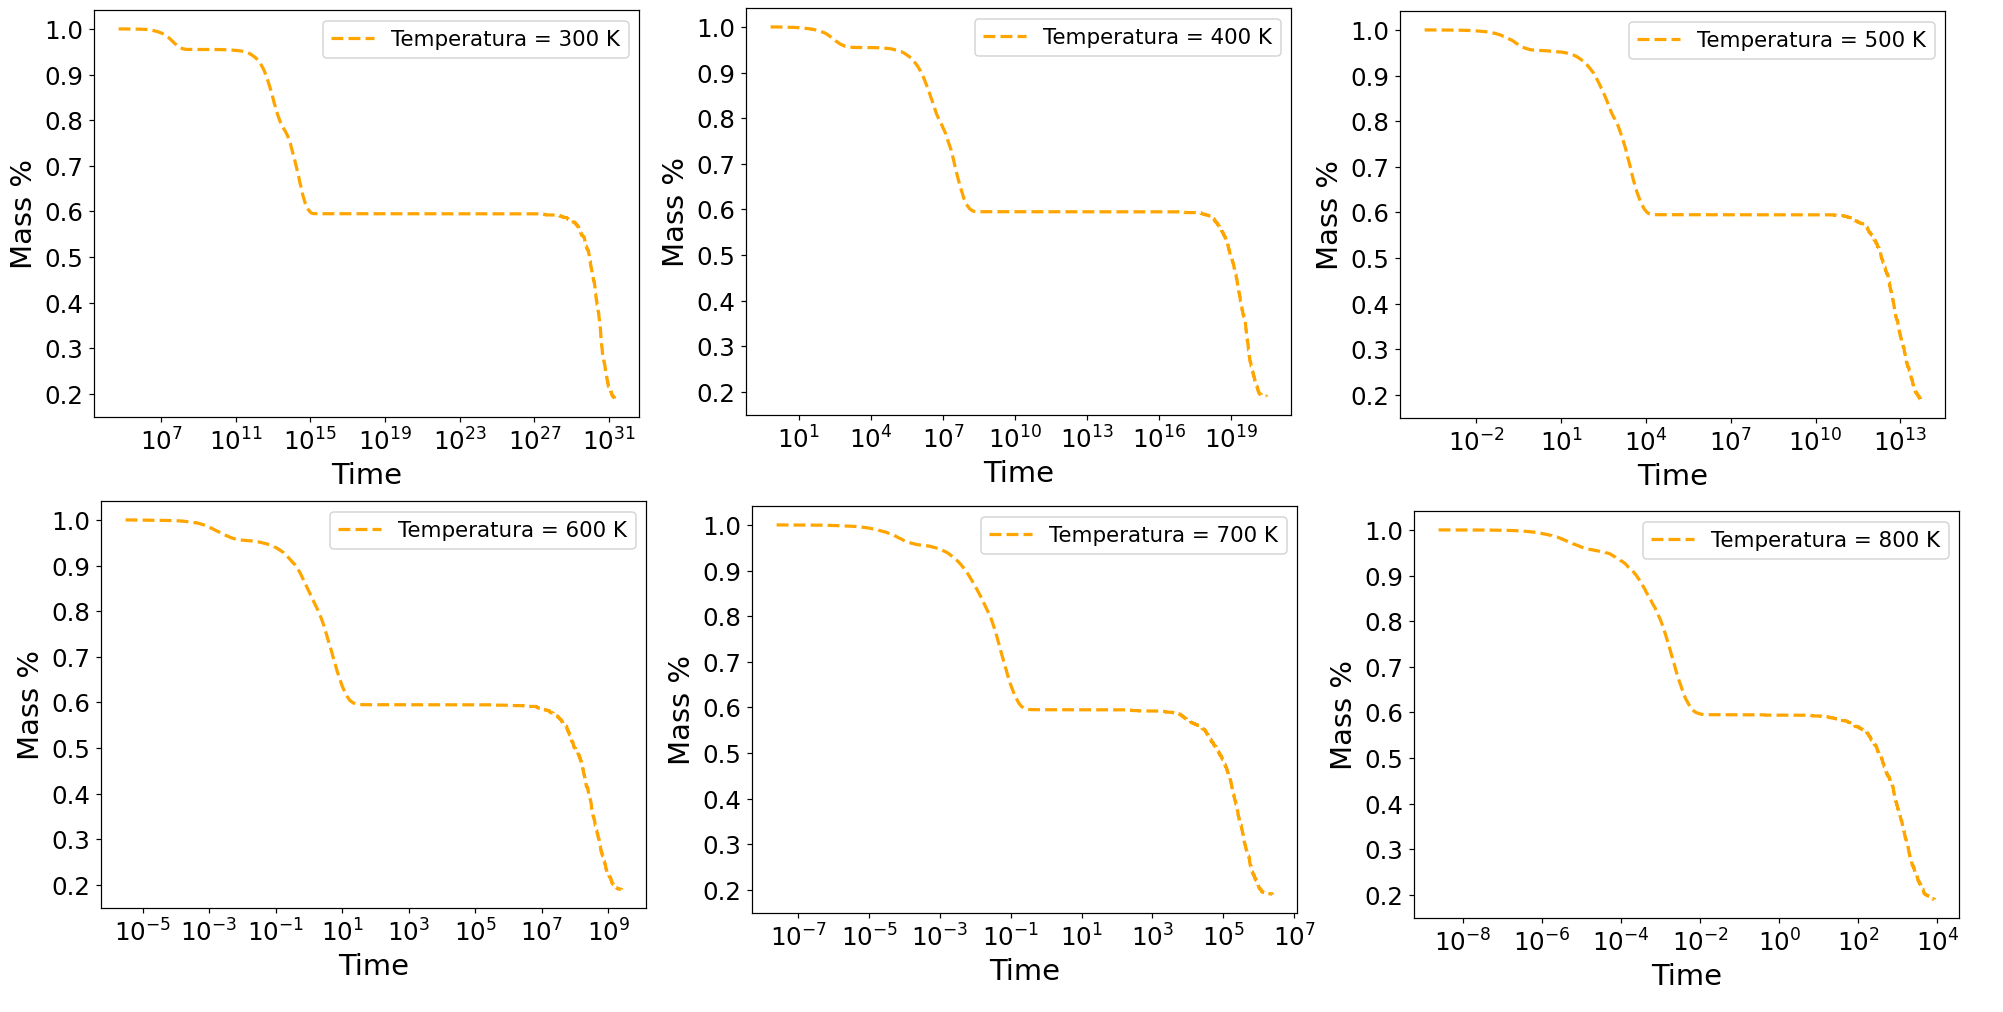
\includegraphics[scale=0.8]{figures/var-massa-tempo-2.png}
\caption{Curva da variação de massa em relação ao tempo obtida através do método de monte carlo cinético para uma superfície com $50\%$ de $0_2$ . }
\label{f2}
\end{figure}

\begin{figure}[!htbp]
%\centering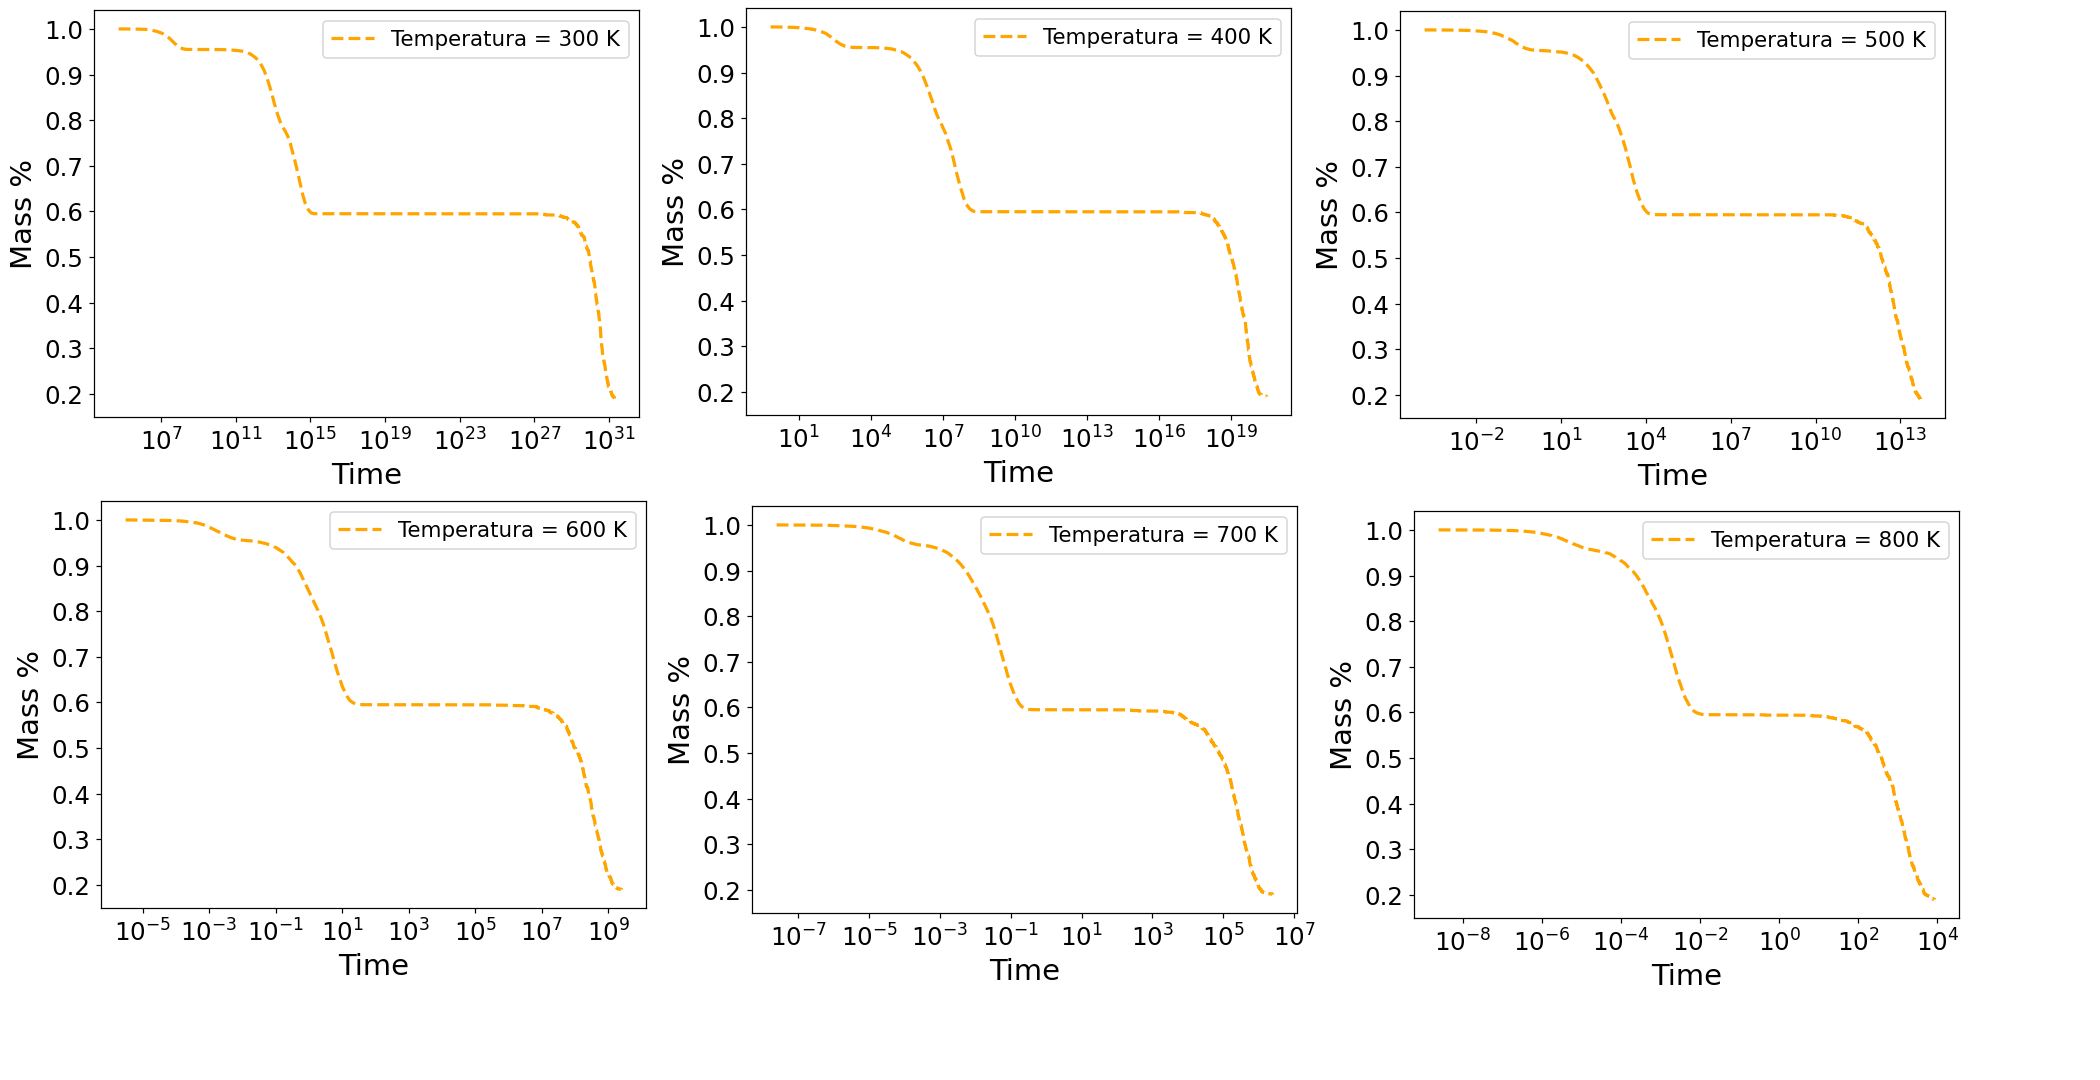
\includegraphics[width=1\linewidth]{figures/var-massa-tempo.png}
\centering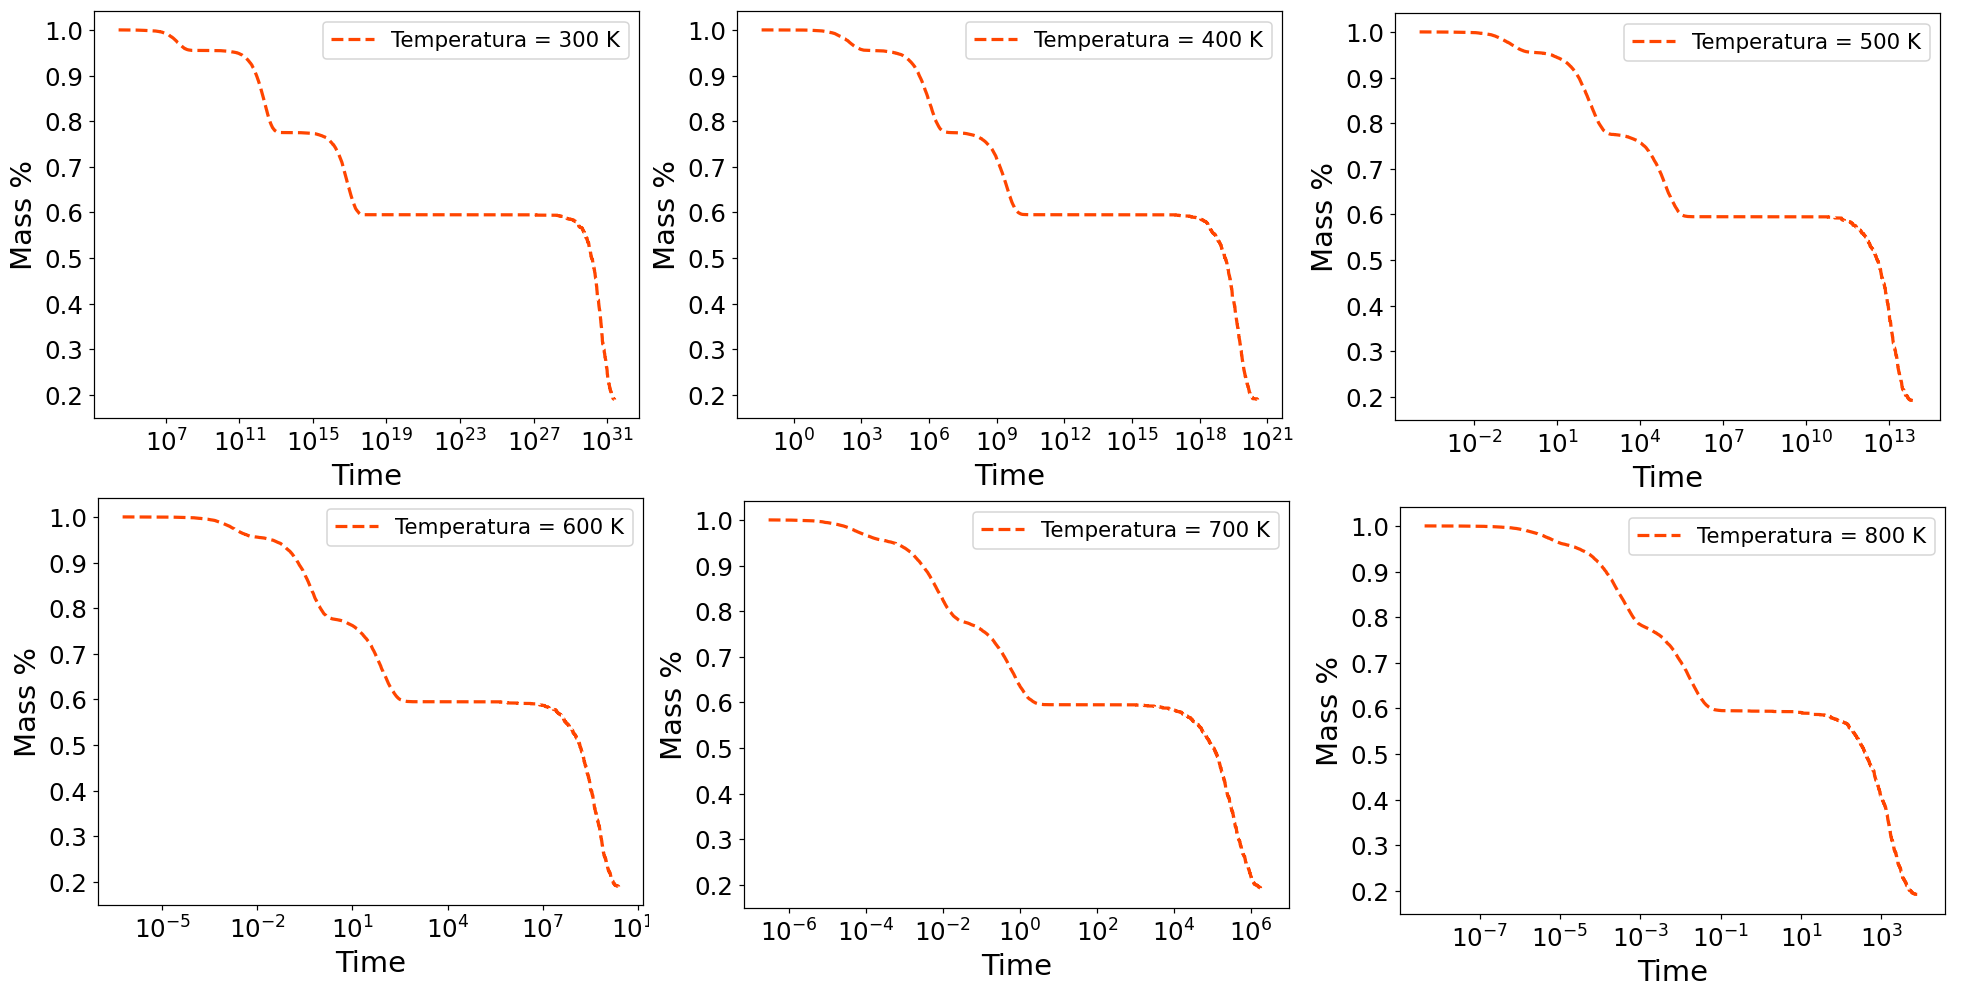
\includegraphics[scale=0.8]{figures/var-massa-tempo-25.png}
\caption{Curva da variação de massa em relação ao tempo obtida através do método de monte carlo cinético para uma superfície com $25\%$ de $0_2$ . }

\label{f3}
\end{figure}

Em seguida,para investigar a dinâmica do sistema de dessorção de átomos de \(S\) do \(TiS_3\) foi aplicado o método de Monte Carlo cinético calculando primeiro a variação de massa em porcentagem ao longo do tempo mantida uma temperatura constante. Este resultado é apresentado nas Figuras \ref{f2} e \ref{f3} onde o modelo considera que o sistema é uma monocamda de \(TiS_3\) exposta a uma Atmosfera com \(50\%\) e \(25\%\) de concentração de \(O_2\) respectivamente. Pode-se ver pelas Figuras \ref{f2} e \ref{f3} que a perda de massa é mais rápida quanto maior for a temperatura considerada para os cálculos.

Além disso, as energias de ativação de cada evento tem participação importante na dinâmica do sistema já que energias maiores terão uma probabilidade menor de acontecer e portanto em geral ocorrerão com maior frequência depois que os eventos de menor energia se tornarem menos prováveis devido por exemplo a diminuição do número de partículas disponíveis para que os eventos de menor energia ocorram. Este comportamento se torna claro quando se analisa a Figura \ref{f3} onde a diferença de energia entre cada evento é maior e observa-se um número maior de degraus no gráfico. Estes degraus denotam quando cada evento ocorre com maior frequência sendo que os de menor energia ocorrem sempre primeiro.

\begin{figure}[!htbp]
%\centering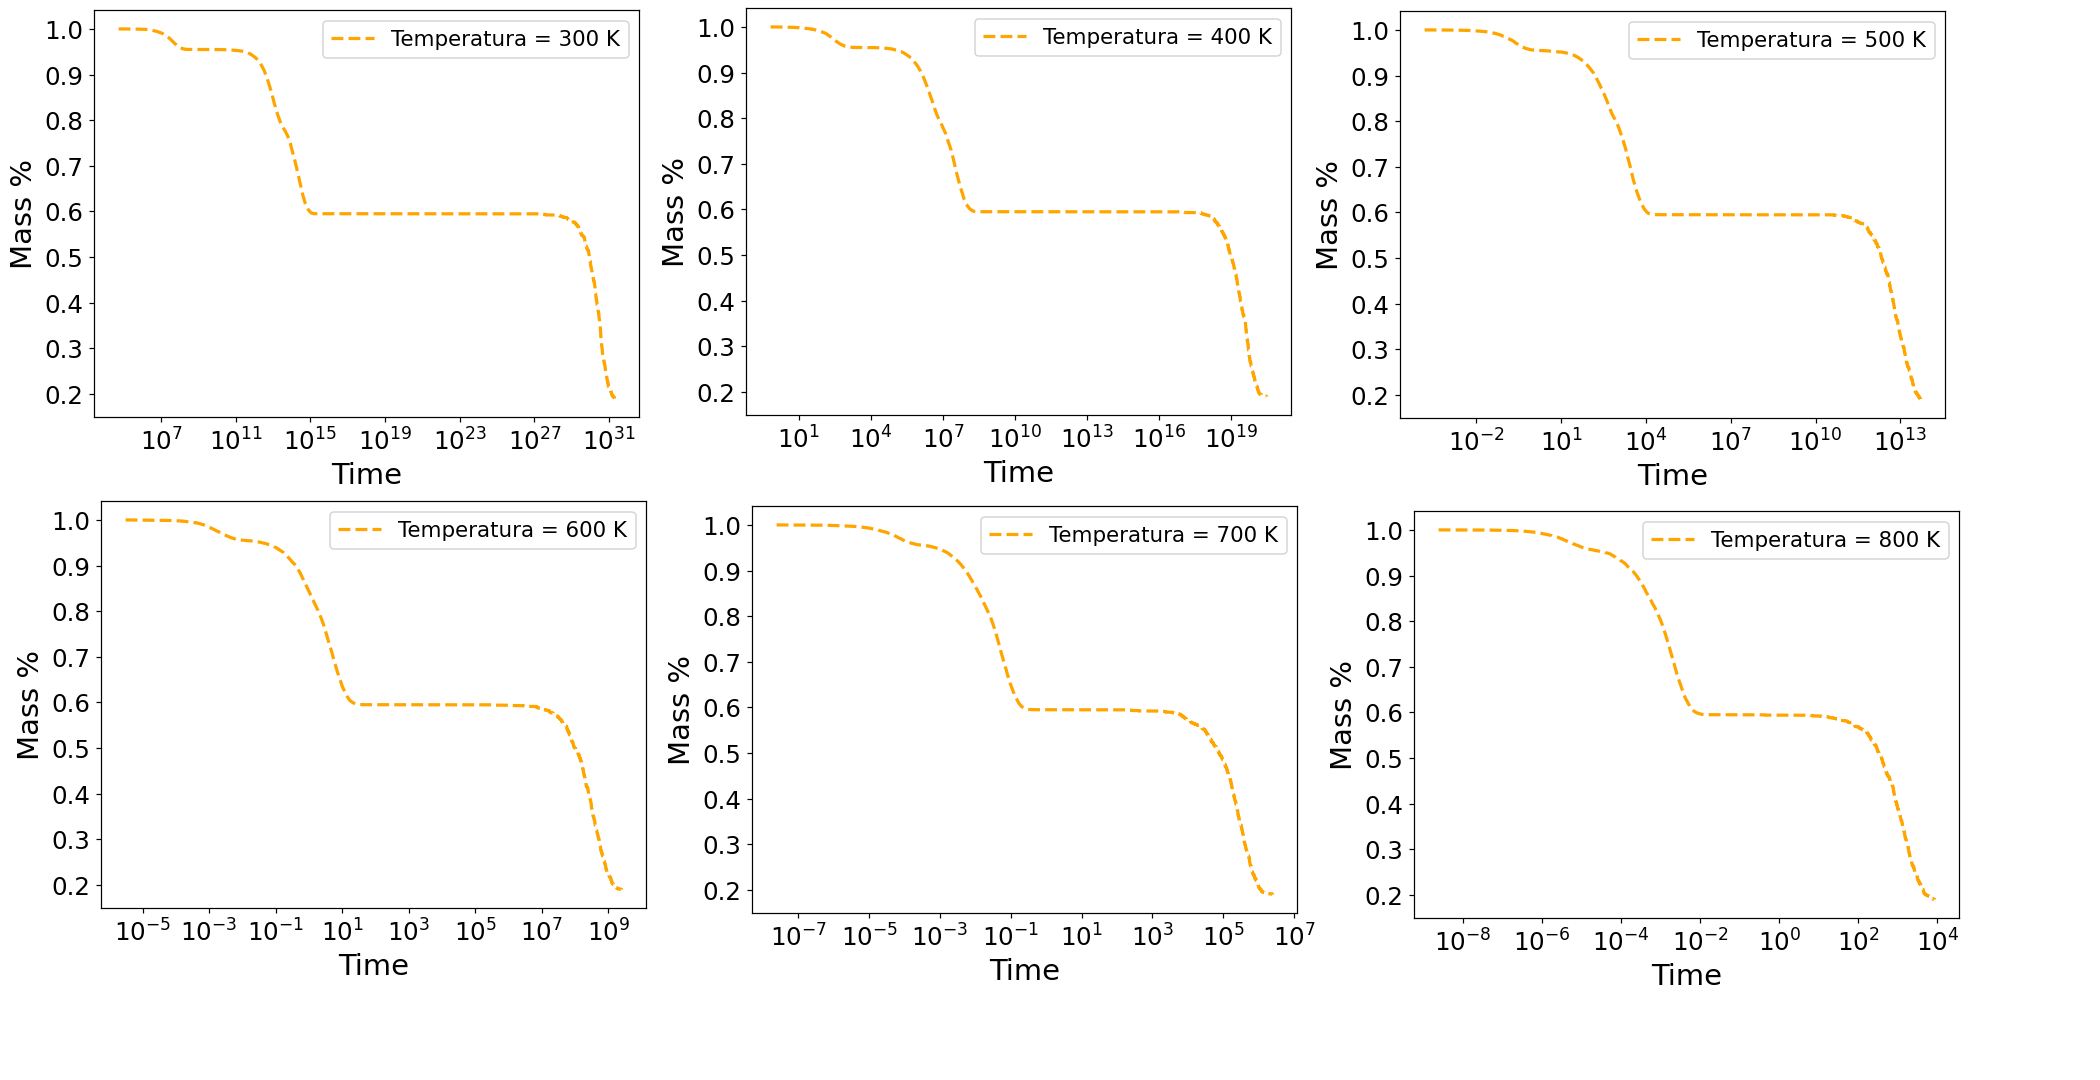
\includegraphics[width=1\linewidth]{figures/var-massa-tempo.png}
\centering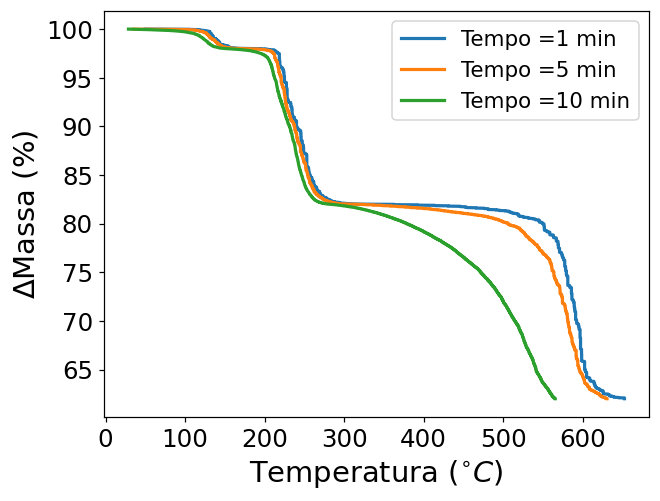
\includegraphics[scale=0.6]{figures/Temperatura-massa.png}
\caption{Curva da variação de massa em relação a temperatura para diferentes intervalos de tempo descritos na legenda, em uma superfície com $50\%$ de $O_2$.}
\label{f4}
\end{figure}


Finalmente, de maneira a comparar os resultados obtidos na curva de termogravimetria apresentada na Figura \ref{f1}, o método de KMC foi utilizado variando a temperatura em escalas de tempo diferentes. Este resultado é apresentado na Figura \ref{f4}. Pode-se ver na Figura \ref{f4} assim como na Figua \ref{f1}, a ocorrência de dois eventos, embora em diferentes intervalos de temperatura. O evento (1) ocorre no intervalo de \(150-250~^\circ C\) com uma variação de massa de \(17.5\%\) que se deve principalmente por formações de monovacâncias e o evento (2) ocorre no intervalo de  \(500-600~^\circ C\) com uma variação de massa de \(21.5\%\) que por sua vez se deve principalmente a formação de divacâncias.

Portanto, o método de KMC concorda razoavelmente bem com a curva de termogravimetria. Este resultado permite concluir que a formação de monovacância e divacâncias podem provocar a degradação do material e consequentemente ocasionar no fenômeno de decomposição elétrica do \(TiS_3\).


\bibliographystyle{ieeetr}
\bibliography{sample.bib}
\end{document}
